\let\negmedspace\undefined
\let\negthickspace\undefined
\documentclass[journal]{IEEEtran}
\usepackage[a5paper, margin=10mm, onecolumn]{geometry}
%\usepackage{lmodern} % Ensure lmodern is loaded for pdflatex

\setlength{\headheight}{1cm} % Set the height of the header box
\setlength{\headsep}{0mm}     % Set the distance between the header box and the top of the text

\usepackage{gvv-book}
\usepackage{gvv}
\usepackage{cite}
\usepackage{amsmath,amssymb,amsfonts,amsthm}
\usepackage{algorithmic}
\usepackage{graphicx}
\usepackage{textcomp}
\usepackage{xcolor}
\usepackage{txfonts}
\usepackage{listings}
\usepackage{enumitem}
\usepackage{mathtools}
\usepackage{gensymb}
\usepackage{comment}
\usepackage[breaklinks=true]{hyperref}
\usepackage{tkz-euclide} 
\usepackage{listings}
\def\inputGnumericTable{}                                 
\usepackage[latin1]{inputenc}                                
\usepackage{color}                                            
\usepackage{array}                                            
\usepackage{longtable}                                       
\usepackage{calc}                                             
\usepackage{multirow}                                         
\usepackage{hhline}                                           
\usepackage{ifthen}                                           
\usepackage{lscape}
\begin{document}

\bibliographystyle{IEEEtran}
\vspace{3cm}

\title{1.2.12}
\author{AI25BTECH11006 - Nikhila}
% \maketitle
% \newpage
% \bigskip
{\let\newpage\relax\maketitle}


\renewcommand{\thefigure}{\theenumi}
\renewcommand{\thetable}{\theenumi}
\setlength{\intextsep}{10pt} % Space between text and floats


\numberwithin{equation}{enumi}
\numberwithin{figure}{enumi}
\renewcommand{\thetable}{\theenumi}


\textbf{Question}:\\

If the points \textbf{A}(6,1),\textbf{B}(8,2),\textbf{C}(9,4) and \textbf{D}(p,3) are the vertices of a parallelogram,taken in order. find the value of p .\\

\vspace{2em}

\textbf{Solution: }

The vector components of the given points $\textbf{A}\begin{pmatrix}6 \\ 1 \end{pmatrix} , \textbf{B}\begin{pmatrix}8 \\ 2\end{pmatrix} , \textbf{C}\begin{pmatrix}9 \\ 4\end{pmatrix}$ and $\textbf{D}\begin{pmatrix}p \\ 3\end{pmatrix}$\\


 If ABCD be a parallelogram with AB $||$ CD ,
 \begin{align}
\textbf{B-A $=$ C-D}
\end{align}


\begin{align}
    \textbf{B}-\textbf{A}=\myvec{8 \\ 2} -\myvec{6 \\ 1}=\myvec{2 \\ 1}\\
    \textbf{C}-\textbf{D}=\myvec{9 \\ 4} -\myvec{p \\ 3}=\myvec{9-p \\ 1} 
\end{align}
By comparing 
\begin{align}
    9-p = 2
\end{align}

We get 
\begin{align}
    p = 7
\end{align}

Hence the coordinates of \textbf{D} are $\myvec{7 \\ 3}$ and the value of p is 7.

\begin{figure}[h!]
   \centering
   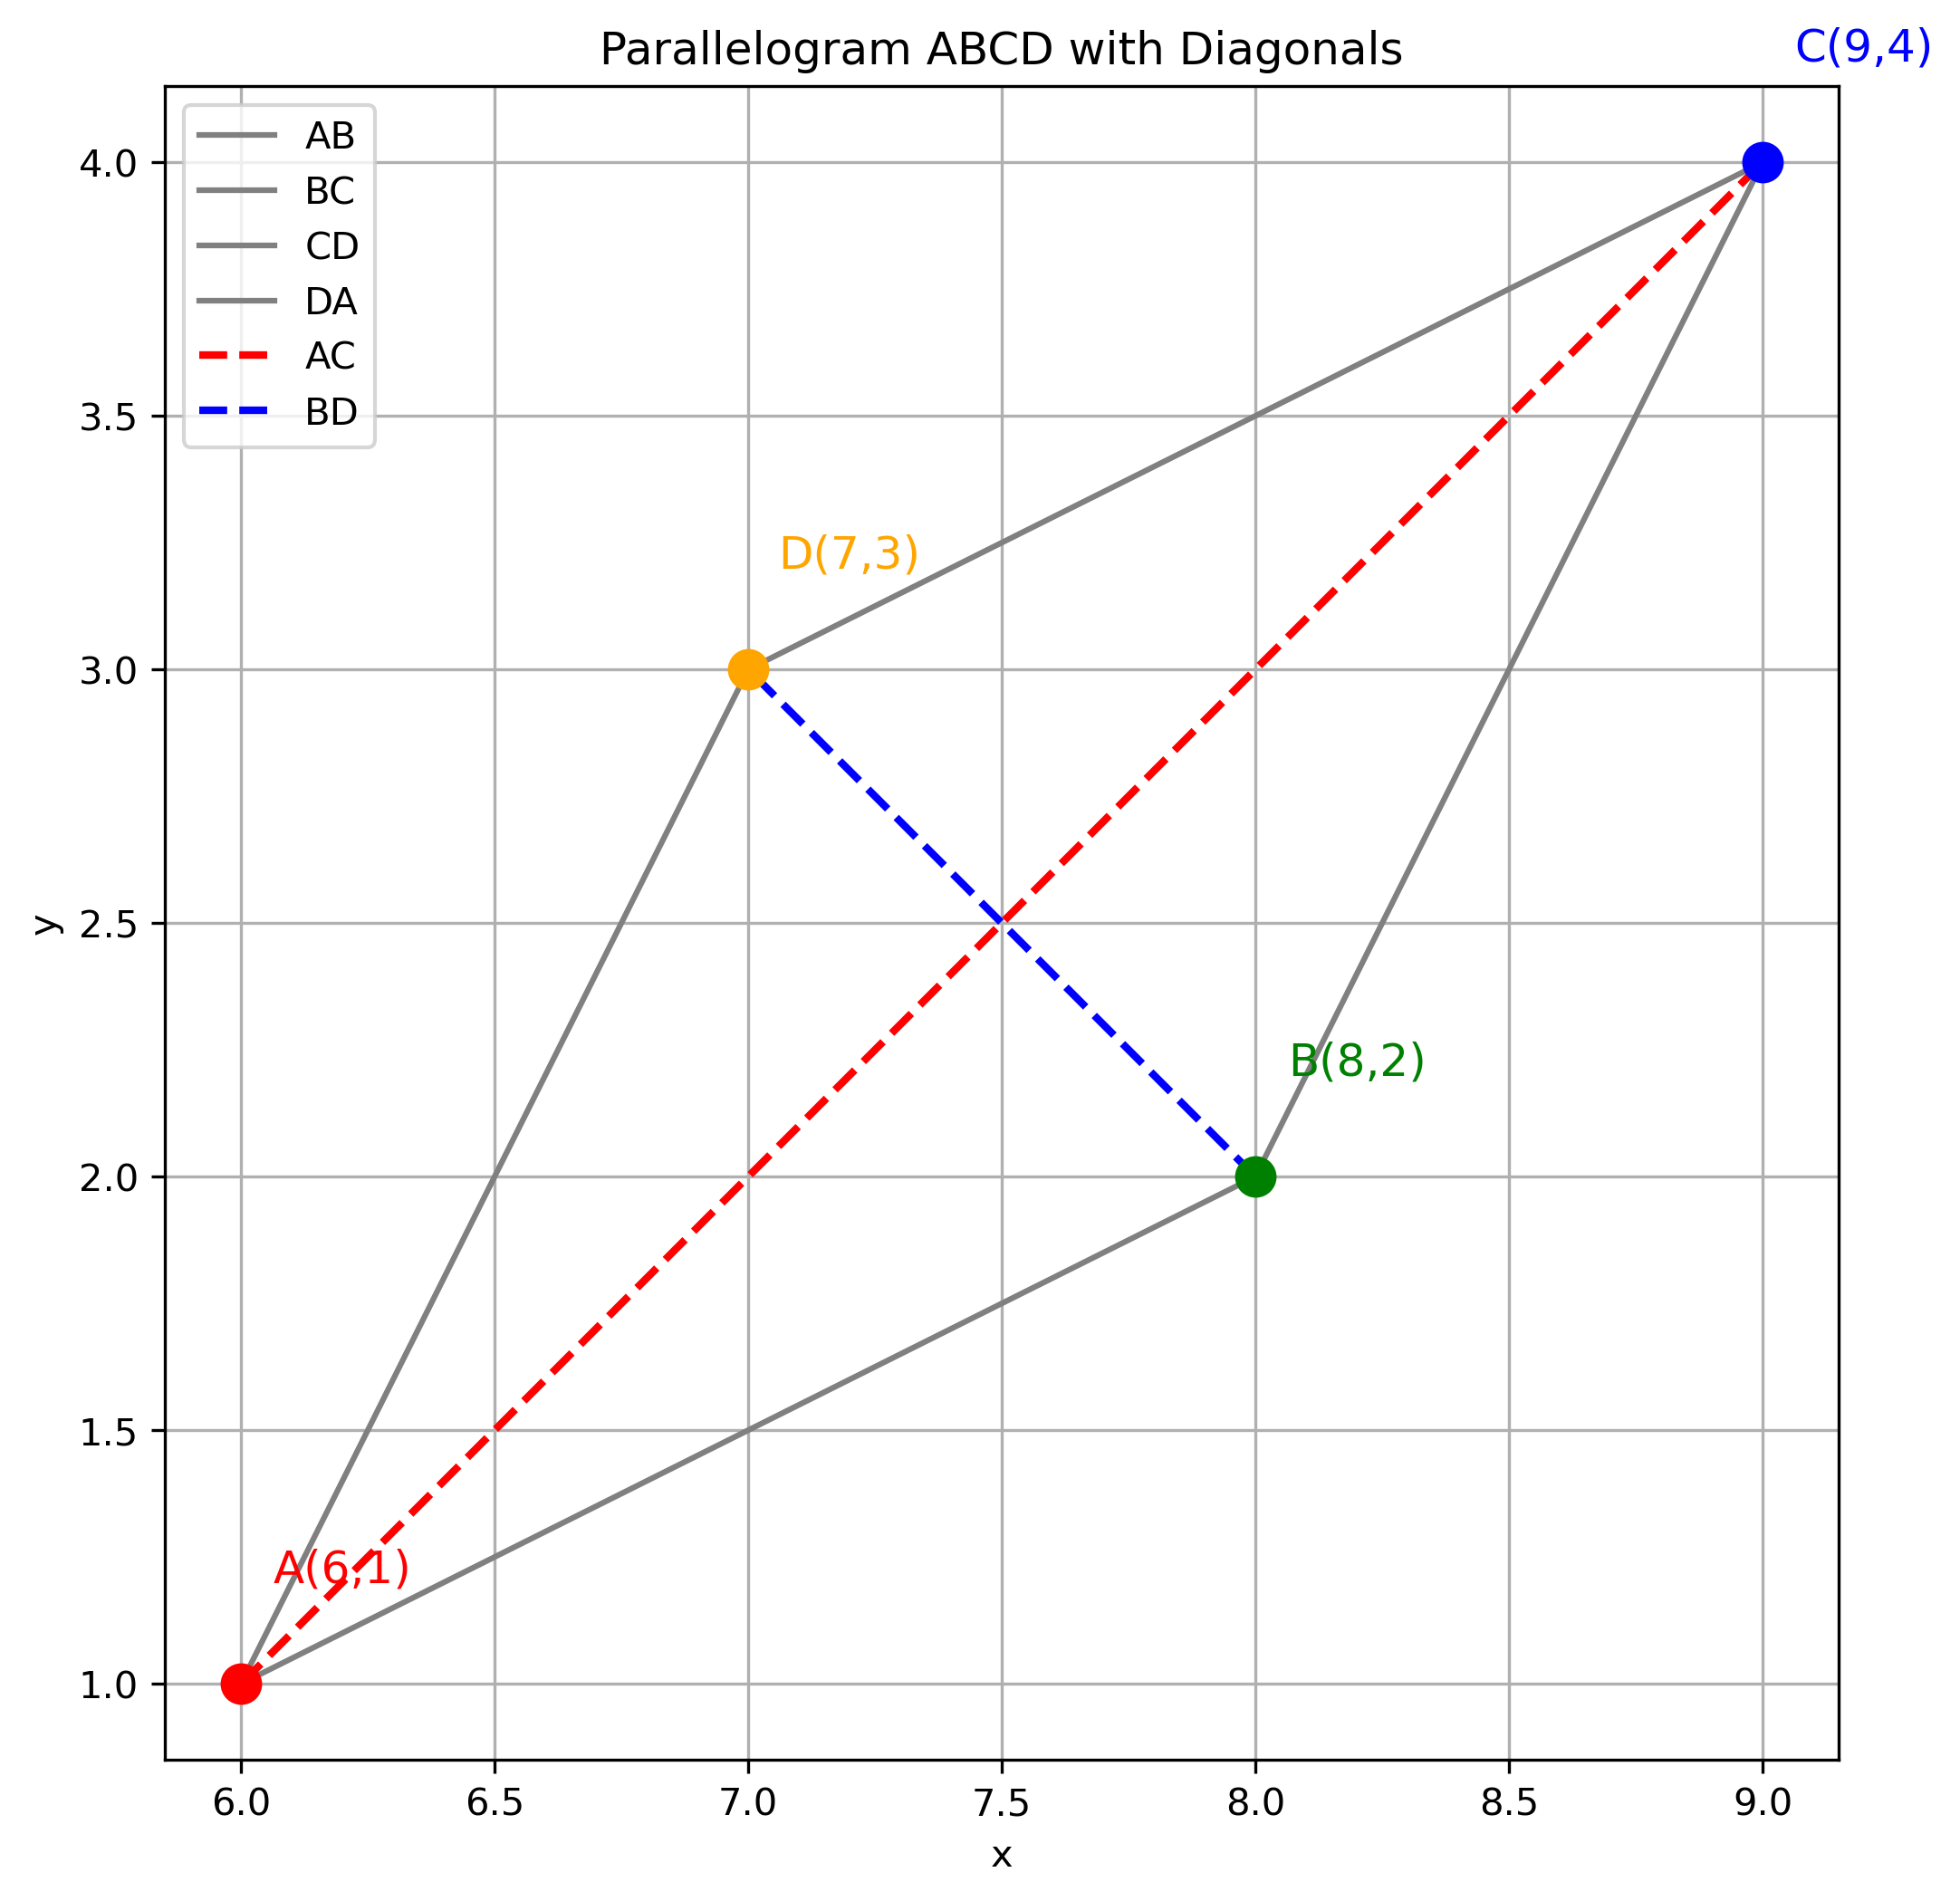
\includegraphics[width=0.7\linewidth]{fig1.png}
   \caption{}
   \label{stemplot}
\end{figure}


\end{document}
